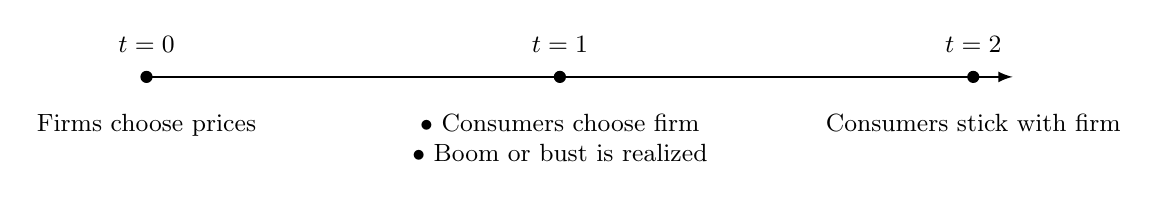
\begin{tikzpicture}[
    >=latex,
    every node/.style={font=\small},
    event/.style={align=center}
]
    % Timeline
    \draw[->,thick] (0,0) -- (11,0);

    % Period markers
    \foreach \x/\t in {0/0,5.25/1,10.5/2} {
        \fill (\x,0) circle (2.2pt);
        \node[above=0.18cm] at (\x,0) {$t=\t$};
    }

    % Events
    \node[event,below=0.35cm] at (0,0)
        {Firms choose prices};
    \node[event,below=0.35cm] at (5.25,0)
        {$\bullet$ Consumers choose firm\\$\bullet$ Boom or bust is realized};
    \node[event,below=0.35cm] at (10.5,0)
        {Consumers stick with firm};
\end{tikzpicture}
